\documentclass[12pt, a4paper]{article}
\usepackage[top=2cm, bottom=2cm, right=2.5cm, left=2.5cm]{geometry}
\usepackage[utf8]{inputenc}
\usepackage{amsmath, amsfonts, amssymb}
\usepackage{float}
\usepackage{graphicx}
\usepackage{multicol}
\usepackage{xcolor}
\usepackage{xwatermark}
\usepackage{setspace}
% \newwatermark[allpages, angle=45, scale=2.0, color=black!15]{matematicautodidata.com}

\title{Homework}
\begin{document}
\begin{minipage}[c][2cm][c]{2cm}

\includegraphics[height=2cm]{logo.pdf}
\end{minipage}
\begin{minipage}[c][3cm][c]{10cm}
\center
{\scriptsize \textit{Sharif University of Technology}}

% {\scriptsize \textit{Department of Mechanical Engineering}}

\textbf{\normalsize Medical Robotics}

{\small{Assignment \#2}}
\smallskip


\end{minipage}
\begin{minipage}[c][3cm][c]{5cm}
\footnotesize
Date: \today

Dr. Behzadipour


\end{minipage}
\vspace{.5cm}

Mohammad Montazeri \hrulefill \, 404205907

\vspace{10pt}

\noindent In this study, the seventh joint of Mitsubishi PA-10 is assumed to be inactive. This actuator controls the manipulator's 7th degree of freedom which is its end-effector's spin; since it does not affect the position of the tool tip, ignoring this motor would not introduce any constraint or conflict. Hence, the reduced 6 DoF manipulator is studied in the following. 

With position of tool tip being fixed, 3 positional constraints act on the robot. The fixed trocar point also adds 2 more positional constraints. With six degrees of freedom, there would not be a unique answer to this problem with 5 constraints. Thus, one can optimize the robot's pose to achieve the best configuration while satisfying the 5 constraints and reaching the desired tool tip and trocar points. After deriving \(x_1\) to \(x_7\) using optimization process, one has elbow and wrist positions as:

\begin{align*}
    P_e^0 = \begin{bmatrix}
        x_e \\
        y_e \\
        z_e 
    \end{bmatrix} = \begin{bmatrix}
        x_1 \\
        x_2 \\
        x_3
    \end{bmatrix} \qquad P_w^0 = \begin{bmatrix}
        x_w \\
        y_w \\
        z_w 
    \end{bmatrix} = \begin{bmatrix}
        x_4 \\
        x_5 \\
        x_6
    \end{bmatrix}
\end{align*}

\section{Inverse Kinematic Model}

After obtaining the vector \(X\), which contains the Cartesian coordinates of the elbow and wrist satisfying the trocar constraint, the corresponding joint variables of the robot must be determined. The inverse geometric model is derived in three successive stages. First, the joint variables \(q_1\) and \(q_2\) are calculated to position the elbow at the desired location. Next, the variables \(q_3\) and \(q_4\) are computed to place the wrist correctly while keeping the first two joints fixed. Finally, the remaining joints \(q_5\) and \(q_6\) are obtained so that the tool tip reaches the required position.

\subsection{Computation of \(q_1\) and \(q_2\)}

The elbow position depends only on the first two joint variables. Considering the geometry of the manipulator, the \(z\)-coordinate of the elbow expressed in frame \(R_0\) can be written as

\begin{align}
z_e^{0} = r_1 + r_3 \cos(q_2)
\end{align}

which yields

\begin{align}
q_2 = \pm \arccos\left(\frac{z_e^{0}-r_1}{r_3}\right)
\end{align}

The projection of the elbow point onto the \(x_0-y_0\) plane provides the first joint angle:

\begin{align}
q_1 = atan2\left(\frac{x_e^{0}}{\sqrt{(x_e^{0})^2 + (y_e^{0})^2}},\frac{x_e^{0}}{\sqrt{(x_e^{0})^2 + (y_e^{0})^2}}\right)
\end{align}

These two variables completely define the elbow configuration.

\subsection{Computation of \(q_3\) and \(q_4\)}

Once \(q_1\) and \(q_2\) are known, the wrist position can be expressed in frame \(R_2\). Let the wrist coordinates obtained from the optimization stage in frame \(R_0\) be denoted by

\begin{align}
P_w^{0} =
\begin{bmatrix}
x_w\\
y_w\\
z_w\\
1
\end{bmatrix}
\end{align}

The homogeneous transformation between frames \(R_2\) and \(R_0\) is constructed using standard rotations and translations:

\begin{align}
T_{2}^0
=
R_z(q_1)\,
T_z(r_1)\,
R_y(q_2)\,
T_z(r_3)
\end{align}

where

\begin{align}
R_z(q_1)=
\begin{bmatrix}
\cos q_1 & -\sin q_1 & 0 & 0\\
\sin q_1 & \cos q_1 & 0 & 0\\
0 & 0 & 1 & 0\\
0 & 0 & 0 & 1
\end{bmatrix}
\end{align}

\begin{align}
R_y(q_2)=
\begin{bmatrix}
\cos q_2 & 0 & \sin q_2 & 0\\
0 & 1 & 0 & 0\\
-\sin q_2 & 0 & \cos q_2 & 0\\
0 & 0 & 0 & 1
\end{bmatrix}
\end{align}

\begin{align}
T_z(r_1)=
\begin{bmatrix}
1 & 0 & 0 & 0\\
0 & 1 & 0 & 0\\
0 & 0 & 1 & r_1\\
0 & 0 & 0 & 1
\end{bmatrix}
\end{align}

\begin{align}
T_x(r_3)=
\begin{bmatrix}
1 & 0 & 0 & 0\\
0 & 1 & 0 & 0\\
0 & 0 & 1 & r_3\\
0 & 0 & 0 & 1
\end{bmatrix}
\end{align}

The wrist coordinates in frame \(R_2\) are then obtained from

\begin{align}
P_w^{2} = T_{0}^{2}\,P_w^{0}
\end{align}

where

\begin{align}
T_{0}^{2} = (T_{2}^{0})^{-1}
\end{align}

By considering the manipulator geometry in frame \(R_2\), the joint variables \(q_3\) and \(q_4\) become

\begin{align}
q_4 = \pm \arccos\left(\frac{z_w^{2}}{r_5}\right)
\end{align}

and

\begin{align}
q_3 = atan2\left({x_w^{2}}, {y_w^{2}}\right)
\end{align}

\subsection{Computation of \(q_5\) and \(q_6\)}

The tool-tip position expressed in frame \(R_4\) is written as

\begin{align}
P_t^{4} =
\begin{bmatrix}
x_t^{4}\\
y_t^{4}\\
z_t^{4}\\
1
\end{bmatrix}
\end{align}

To obtain this quantity, the homogeneous transformation from frame \(R_4\) to frame \(R_0\) must first be determined. Using the same sequence of homogeneous rotations and translations, the transformation matrix is expressed as

\begin{align}
T_{4}^{0}
=
R_z(q_1)\,
T_z(r_1)\,
R_y(q_2)\,
T_z(r_3)\,
R_z(q_3)\,
R_y(q_4)\,
T_z(r_5)
\end{align}

Thus,

\begin{align}
P_t^{4} = T_0^{4}\,P_t^{4}
\end{align}

with

\begin{align}
T_0^{4} = (T_4^{0})^{-1}
\end{align}

The remaining joint variables are then obtained from the projection of the tool-tip position in frame \(R_4\):

\begin{align}
q_6 = \pm \arccos\left(\frac{z_t^{4}}{r_7}\right)
\end{align}

and

\begin{align}
q_5 = \arctan\left({x_t^{4}}, {y_t^{4}}\right)
\end{align}

Consequently, all joint variables required to satisfy the penetration point constraint are determined from the elbow, wrist, and tool-tip Cartesian coordinates.

\section{Discussion and Conclusion}
In this work, the Mitsubishi PA-10 manipulator was considered effectively as a six-degree-of-freedom robot since the seventh joint only produces axial rotation of the end-effector and does not affect the tooltip position. The surgical task imposes five independent constraints on the system. Three constraints arise from fixing the tooltip position in Cartesian space, while the trocar condition contributes two additional constraints because constraining a point to remain on a line removes only two independent spatial directions. Therefore, the robot still possesses one remaining degree of redundancy, allowing multiple robot configurations to satisfy the same tooltip trajectory and trocar constraint. Physically, this redundancy corresponds to the elbow swivel motion around the line connecting the shoulder, trocar point, and tooltip.

For a general six-degree-of-freedom serial robot, the inverse kinematics problem may admit multiple discrete solutions due to different elbow-up/elbow-down and wrist configurations. In the present problem, the trocar constraint reduces the admissible configuration space but does not eliminate redundancy completely. Consequently, the inverse kinematics problem under the trocar constraint still possesses infinitely many feasible solutions associated with the remaining redundant degree of freedom. In practice, however, the optimization algorithm converges to one specific solution depending on the initial guess, numerical tolerances, and continuity of the trajectory.

Although the paper formulates seven scalar equations, these equations do not represent seven independent physical constraints. Instead, they are part of an intermediate geometric reconstruction problem used to determine the elbow and wrist positions before solving the inverse kinematics. Some of these equations are geometrically dependent and therefore redundant. In the present implementation, the constraint equations were solved using a Levenberg-Marquardt nonlinear least-squares optimization in MATLAB, leading to the following results. The Matlab live script code is also appended to this report.



\begin{figure}[htbp]
    \centering
    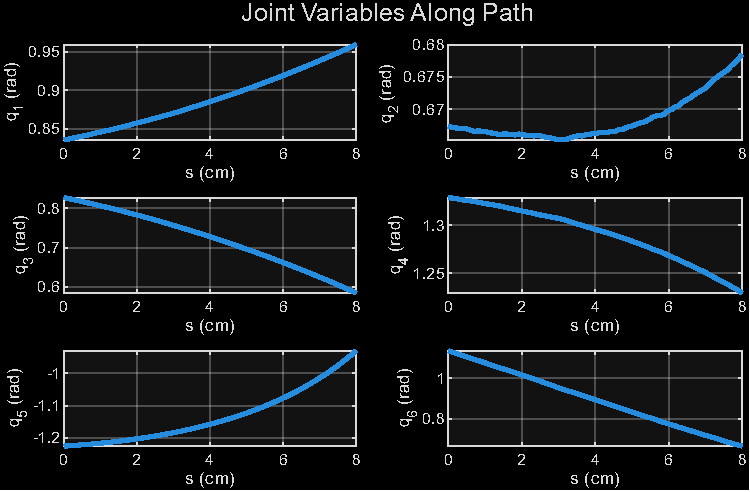
\includegraphics[width=.85\textwidth]{Figure1.pdf}
    \caption{Joint-variable plots \(q_1\) to \(q_6\) versus path parameter \(s\).}
    \label{fig:pic1}
\end{figure}

\begin{figure}[htbp]
    \centering
    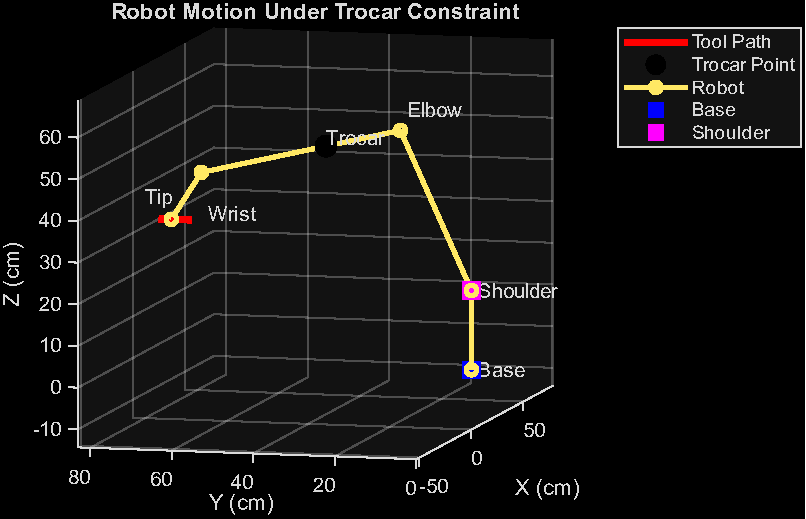
\includegraphics[width=.85\textwidth]{Figure2.pdf}
    \caption{A 3D snapshot of the robot mid-path.}
    \label{fig:pic2}
\end{figure}

% \begin{align}
%     \theta_1 =& \operatorname{atan}2\left(\frac{x}{\sqrt{x^2+z^2}}, \frac{-z}{\sqrt{x^2+z^2}}\right) \label{eq:pos-start}\\
%     \theta_3=&\cos^{-1} \frac{X^2+Y^2-l_2^2-{l_3^\prime}^2}{2 l_2 {l_3^\prime}} \rightarrow \left\{\begin{array}{l}
% \theta_3^1 \\
% \\
% \theta_3^2
% \end{array}\right. 
% \end{align}


\begin{thebibliography}{99}

\bibitem{Michelin2002}
M.~Michelin, E.~Dombre, P.~Poignet, F.~Pierrot, and L.~Eckert,
``Path Planning under a Penetration Point Constraint for Minimally Invasive Surgery,''
in \textit{Proceedings of the IEEE/RSJ International Conference on Intelligent Robots and Systems (IROS)}, Lausanne, Switzerland, 2002, pp.~1475--1480.

\end{thebibliography}




\end{document}